\section{Three dimensions: further results}\label{supp:three}

\paragraph{The gate of the three-dimensional comparison}
The gate of the three-dimensional comparison combined three conditions as (a) and ((b) or
(c)) (\cref{tab:criteria}): (a) a sanity check on the supervised side, (b) the label-free
transformer's displacement error within 10\% of the displacement-supervised transformer's
with 1,024 labels and an advantage in relative energy gap of at least 40\% at every budget,
and (c) transfer to the finer mesh. Condition (b), the pre-registered test of the label-free
network's accuracy, was met with a wide margin: the label-free displacement error was
\numGTwoParity{} relative to the displacement-supervised one, and the smallest advantage in
relative energy gap was \numGTwoAdvMin{}; the kill conditions on that accuracy, KP1 and KP2,
were not triggered. Condition (c) failed, and kill condition KP4 withdrew the transfer claim
(Section~\ref{sec:transfer}). Condition (a) was met from 64 labels on, but with 16 labels
the displacement-supervised transformer with the energy term was only
\numGTwoSanitySixteen{} times more accurate in displacement than the zero field, against the
\numGTwoSanityX{} required. The amendment, written after this result of the initial run was
known, assessed (a) only from \numGTwoFloor{} labels: under it the gate read GO, and under
the registered form, which assesses every budget, it read NO-GO (Section~\ref{app:prereg}).
The claims of the paper rest on condition (b) and on the measurements, not on the gate's
verdict.

\paragraph{The displacement-supervised transformer's seed means}
The displacement-supervised transformer's mean relative energy gap, \numThreeLabGapMs{}, is
the mean of three seeds, \numThreeLabGapSeeds{}. The second is dominated by validation
instance No.~\numWorstIndex{}, whose prediction in seed \numThreeLabWorstSeed{} had a
relative energy gap of \numThreeLabWorst{}, averaged over its four load cases, with a
displacement error of \numWorstSeedLabDisp{}, a von Mises error of \numWorstSeedLabVm{} and
a peak stress error of \numWorstSeedLabPeak{}. The same instance had the largest relative
energy gap of the displacement-supervised transformer in all three seeds, and its median
relative energy gap, \numThreeLabGapMedian{}, is far below its mean. The energy term
repaired most of this, but not at every budget: with 256 labels it raised the displacement
error of the displacement-supervised transformer in every seed and, through one of the three
seeds, its mean relative energy gap (\cref{tab:labeleff}), although it reduced the number of
instance-seed predictions worse than the zero field from \numThreeLabWorseTwoFiveSix{} to
\numThreeAncWorseTwoFiveSix{}.

\paragraph{Fewer labels}
\Cref{tab:labeleff} gives the values that \cref{fig:labeleff} plots, in both dimensions,
with the networks of the two-dimensional comparison; the values of the July run are in
Section~\ref{app:july}.

% generated from the committed records; do not edit
\begin{table}[tbp]
\centering
\footnotesize
\setlength{\tabcolsep}{4pt}
\caption{Label efficiency: relative displacement error / relative energy gap against the number of labelled training instances (seed means).}
\label{tab:labeleff}
\resizebox{\ifdim\width>\textwidth\textwidth\else\width\fi}{!}{%
\begin{tabular}{llcccc}
\toprule
Run & Model & 16 & 64 & 256 & 1,024 \\
\midrule
3D & Supervised & 0.395 / 18.5 & 0.288 / 5.95 & 0.0726 / 0.799 & 0.0470 / 31.2 \\
3D & Supervised + energy term & 0.369 / 0.621 & 0.256 / 0.854 & 0.0833 / 0.964 & 0.0470 / 0.116 \\
3D & Graph network, supervised & -- & 0.149 / 18.3 & -- & 0.0168 / 0.447 \\
3D & Nearest-neighbour field & 0.648 / 5.74 & 0.477 / 2.24 & 0.400 / 1.20 & 0.382 / 1.22 \\
3D & Label-free (no labels) & 0.0300 / 0.00912 & 0.0300 / 0.00912 & 0.0300 / 0.00912 & 0.0300 / 0.00912 \\
\midrule
2D & Supervised & 0.459 / 20.8 & 0.165 / 3.06 & 0.0712 / 0.430 & 0.0505 / 0.133 \\
2D & Supervised, stiffness norm & 0.362 / 0.254 & 0.0889 / 0.0505 & 0.0667 / 0.0383 & 0.0547 / 0.0290 \\
2D & Graph network, supervised & -- & 0.370 / 149 & -- & 0.0499 / 0.825 \\
2D & Nearest-neighbour field & 0.687 / 6.50 & 0.466 / 1.65 & 0.408 / 1.03 & 0.404 / 0.959 \\
2D & Label-free (no labels) & 0.0634 / 0.0383 & 0.0634 / 0.0383 & 0.0634 / 0.0383 & 0.0634 / 0.0383 \\
\bottomrule
\end{tabular}}

\smallskip
\begin{minipage}{\linewidth}\footnotesize\raggedright
Seed means over 3 seeds; the nearest-neighbour field is deterministic. A dash marks a budget at which the model was not trained (the graph network was trained at 64 and 1,024 labels only). 3D: the three-dimensional comparison (\cref{tab:3d}); 2D: the two-dimensional comparison (\cref{tab:2d}). The label-free row repeats its single value, which uses the same 1,024 instances without labels.
\end{minipage}
\end{table}


\paragraph{The three-dimensional energy-norm run}
\Cref{tab:k3d} gives the pre-registered hypotheses of the run with their per-seed values and
the readings that its pre-registration required beside each verdict. \Cref{tab:kmedians}
gives every metric of the three transformers on the 256 validation instances, as the seeds'
medians over the instances, the statistic that the verdicts read, and as the seeds' means.
\Cref{tab:kcomparisons} gives the \numKdSecondary{} secondary comparisons that the
pre-registration fixed as exploratory readings, without a criterion: for each of the five
metrics, the energy-norm-supervised transformer against the displacement-supervised and the
label-free transformers, and the label-free transformer against the displacement-supervised
one, on the medians and on the means. Each reading applies the noise guard of the paper: rel
is the relative difference of the two networks' seed-averaged values, and a difference
counts only beyond the larger of 10\% and twice its standard error over the three seeds.
Without a true difference, a comparison can cross the guard by chance, as the
pre-registration's simulations of the rule show, so several crossings among
\numKdSecondary{} are expected by chance. For the critical-region recall higher is better,
and the reading says which network was the better. Descriptively, on the medians, the change
of norm removed \numKdClosureVm{} of the displacement-supervised transformer's excess over
the label-free transformer in von Mises error and \numKdClosureGap{} in relative energy gap,
a reading that the pre-registration fixed without a criterion. The energy-norm-supervised
and the displacement-supervised transformers were trained about seven weeks apart, each with
the code of its time, whose training path a regression on small problems showed to be the
same; the stored networks were evaluated again with the later code and reproduced their
earlier values exactly.

% generated from the committed records; do not edit
\begin{table}[tbp]
\centering
\footnotesize
\setlength{\tabcolsep}{4pt}
\caption{The pre-registered hypotheses of the three-dimensional energy-norm run, with 1,024 labelled instances, as its adjudicator recorded them, and the readings its pre-registration required beside each.}
\label{tab:k3d}
\resizebox{\ifdim\width>\textwidth\textwidth\else\width\fi}{!}{%
\begin{tabular}{lccc}
\toprule
 & H2a-3D & H2b-3D & H3-3D \\
\midrule
Network A & Supervised, energy norm & Supervised, energy norm & Supervised, energy norm \\
Reference B & Supervised ($\mathcal{L}_D$) & Supervised ($\mathcal{L}_D$) & Label-free \\
Metric & Relative energy gap & von Mises error & Relative energy gap \\
\midrule
A, seeds 0, 1, 2 & 0.00432, 0.00448, 0.00452 & 0.0412, 0.0425, 0.0437 & 0.00432, 0.00448, 0.00452 \\
B, seeds 0, 1, 2 & 0.224, 0.256, 0.275 & 0.247, 0.254, 0.276 & 0.00932, 0.00744, 0.00581 \\
\midrule
rel & $-$98.2\% & $-$83.6\% & $-$41.0\% \\
SE$_\mathrm{rel}$ & 5.9\% & 3.4\% & 13.5\% \\
Guard & 11.7\% & 10.0\% & 27.0\% \\
Reading & supported & supported & A lower \\
\midrule
Welch 95\% interval & $-$123.5\% to $-$73.0\% & $-$98.0\% to $-$69.2\% & $-$98.7\% to +16.7\% \\
Instance resampling 95\% & $-$98.4\% to $-$98.1\% & $-$84.5\% to $-$82.7\% & $-$43.9\% to $-$38.4\% \\
\midrule
Seed means: rel (guard) & $-$99.98\% (guard 197.9\%) & $-$88.1\% (guard 43.7\%) & $-$44.7\% (guard 29.0\%) \\
Seed means: Welch 95\% & $-$526\% to +326\% & $-$182\% to +6\% & $-$106\% to +16\% \\
\midrule
Holdout: rel (guard) & $-$98.0\% (guard 12.6\%) & $-$83.0\% (guard 10.0\%) & $-$38.0\% (guard 25.6\%) \\
Holdout, seed means: rel (guard) & $-$99.997\% (guard 199.6\%) & $-$89.0\% (guard 60.2\%) & $-$35.4\% (guard 26.4\%) \\
\bottomrule
\end{tabular}}

\smallskip
\begin{minipage}{\linewidth}\footnotesize\raggedright
Every reading is of the seeds' values, each seed's median over the 256 validation instances (the pre-registered statistic) unless the row says seed means; rel, SE$_\mathrm{rel}$ and the noise guard as defined in the note to \cref{tab:criteria}. Welch: rel $\pm$ t $\times$ SE$_\mathrm{rel}$ at the Welch--Satterthwaite degrees of freedom, a symmetric interval that can extend below $-$100\%. Instance resampling: the 2.5\% and 97.5\% percentiles of rel over 2,000 resamplings of the 256 instances, the same instances for both networks and every seed, the seeds kept, each seed's value the median of its resampled values. Holdout: the same readings on the 686 held-out instances of \cref{sec:holdout}, without a verdict.\par
H3-3D is a reading without a criterion. With the roles of A and B exchanged, rel was +69.5\% against a guard of 45.8\%.
\end{minipage}
\end{table}


% generated from the committed records; do not edit
\begin{table}[tbp]
\centering
\footnotesize
\setlength{\tabcolsep}{4pt}
\caption{Three-dimensional stiffness-norm run: every metric of the three transformers on the 256 validation instances, the seeds' medians and the seeds' means over the instances (mean $\pm$ sample standard deviation over the three seeds).}
\label{tab:kmedians}
\resizebox{\ifdim\width>\textwidth\textwidth\else\width\fi}{!}{%
\begin{tabular}{llccccc}
\toprule
Network & Statistic & \shortstack{Displacement \\ error} & \shortstack{Relative \\ energy gap} & \shortstack{von Mises \\ error} & \shortstack{Peak stress \\ error} & \shortstack{Critical-region \\ recall} \\
\midrule
Label-free & seed medians & 0.0271 $\pm$ 0.0022 & 0.00752 $\pm$ 0.00176 & 0.0527 $\pm$ 0.0040 & 0.0785 $\pm$ 0.0149 & 0.790 $\pm$ 0.023 \\
 & seed means & 0.0300 $\pm$ 0.0028 & 0.00912 $\pm$ 0.00228 & 0.0554 $\pm$ 0.0045 & 0.0807 $\pm$ 0.0134 & 0.793 $\pm$ 0.022 \\
\midrule
Supervised ($\mathcal{L}_D$) & seed medians & 0.0415 $\pm$ 0.0026 & 0.251 $\pm$ 0.026 & 0.259 $\pm$ 0.015 & 0.222 $\pm$ 0.014 & 0.628 $\pm$ 0.009 \\
 & seed means & 0.0470 $\pm$ 0.0038 & 31.2 $\pm$ 53.5 & 0.370 $\pm$ 0.140 & 0.784 $\pm$ 0.807 & 0.619 $\pm$ 0.005 \\
\midrule
Supervised, stiffness norm & seed medians & 0.0203 $\pm$ 0.0019 & 0.00444 $\pm$ 0.00010 & 0.0425 $\pm$ 0.0013 & 0.0379 $\pm$ 0.0008 & 0.858 $\pm$ 0.001 \\
 & seed means & 0.0227 $\pm$ 0.0022 & 0.00504 $\pm$ 0.00022 & 0.0440 $\pm$ 0.0014 & 0.0386 $\pm$ 0.0011 & 0.858 $\pm$ 0.001 \\
\bottomrule
\end{tabular}}
\end{table}


% generated from the committed records; do not edit
\begin{table}[tbp]
\centering
\footnotesize
\setlength{\tabcolsep}{4pt}
\caption{Three-dimensional stiffness-norm run: the 30 secondary comparisons, exploratory, each with the noise guard, on the seeds' medians and on the seeds' means.}
\label{tab:kcomparisons}
\resizebox{\ifdim\width>\textwidth\textwidth\else\width\fi}{!}{%
\begin{tabular}{llcccc}
\toprule
Comparison (A against B) & Metric & Medians: rel (guard) & Reading & Seed means: rel (guard) & Reading \\
\midrule
Stiffness norm against supervised ($\mathcal{L}_D$) & Displacement error & $-$51.1\% (guard 10.0\%) & A better & $-$51.8\% (guard 10.8\%) & A better \\
 & Relative energy gap & $-$98.2\% (guard 11.7\%) & A better & $-$99.98\% (guard 197.9\%) & within \\
 & von Mises error & $-$83.6\% (guard 10.0\%) & A better & $-$88.1\% (guard 43.7\%) & A better \\
 & Peak stress error & $-$82.9\% (guard 10.0\%) & A better & $-$95.1\% (guard 118.9\%) & within \\
 & Critical-region recall & +36.7\% (guard 10.0\%) & A better & +38.6\% (guard 10.0\%) & A better \\
\midrule
Stiffness norm against label-free & Displacement error & $-$25.0\% (guard 12.3\%) & A better & $-$24.3\% (guard 13.7\%) & A better \\
 & Relative energy gap & $-$41.0\% (guard 27.0\%) & A better & $-$44.7\% (guard 29.0\%) & A better \\
 & von Mises error & $-$19.4\% (guard 10.0\%) & A better & $-$20.6\% (guard 10.0\%) & A better \\
 & Peak stress error & $-$51.7\% (guard 22.0\%) & A better & $-$52.1\% (guard 19.2\%) & A better \\
 & Critical-region recall & +8.7\% (guard 10.0\%) & within & +8.1\% (guard 10.0\%) & within \\
\midrule
Label-free against supervised ($\mathcal{L}_D$) & Displacement error & $-$34.7\% (guard 10.0\%) & A better & $-$36.3\% (guard 11.6\%) & A better \\
 & Relative energy gap & $-$97.0\% (guard 11.8\%) & A better & $-$99.97\% (guard 197.9\%) & within \\
 & von Mises error & $-$79.6\% (guard 10.0\%) & A better & $-$85.0\% (guard 43.7\%) & A better \\
 & Peak stress error & $-$64.6\% (guard 10.6\%) & A better & $-$89.7\% (guard 118.9\%) & within \\
 & Critical-region recall & +25.8\% (guard 10.0\%) & A better & +28.2\% (guard 10.0\%) & A better \\
\bottomrule
\end{tabular}}
\end{table}


\paragraph{A typical instance}
\Cref{fig:field-median} shows the validation instance with the median relative energy gap of
the label-free transformer, on which the predictions of the networks trained on the
displacement error were better than the zero field and their stress fields still rough.

\begin{figure}[tbp]
\centering
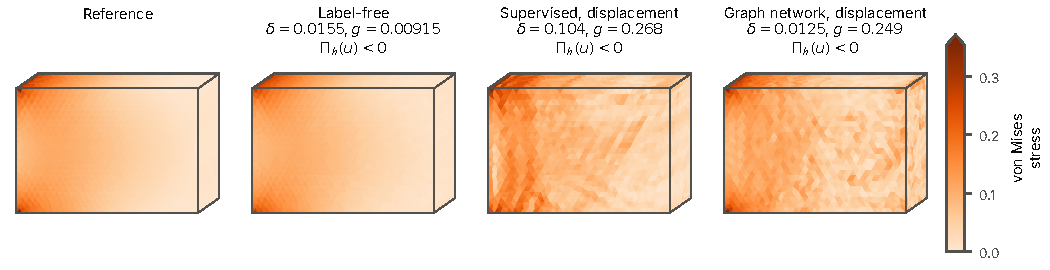
\includegraphics[width=\linewidth]{generated/fig_field_median.pdf}
\caption{A typical validation instance, the one with the median relative energy gap of the
label-free transformer, seed 0, under the \numFigMedianLoad{} (selection rules in
Section~\ref{app:repro:plots}). Von Mises stress of the reference solution and of the three
networks, displayed as in \cref{fig:field-worst}.}
\label{fig:field-median}
\end{figure}
